\chapter{El experimento \label{chap:ConfiguracionExperimental}}
%%%%%%%%%%%%%%%%%%%%%%%%%%%%%%%%%%%%%%%%%%%%%%%%%%%%%%%%%%%%%%%%%%
%%%%%%%%%%%%%%%%%%%%%%%%%%%%%%%%%%%%%%%%%%%%%%%%%%%%%%%%%%%%%%%%%%

\noindent En este capítulo se describe el experimento realizado en Fermilab\footnote{Laboratorio Nacional de Aceleradores Fermi en Estados Unidos} para la obtención de los datos utilizados en esta tesis. Si bien el experimento no formó parte de este trabajo, como se verá más adelante, su descripción se vuelve necesaria para explicar algunos de los fenómenos observados.

\section{Configuración experimental}
\noindent Se describe a continuación el sistema utilizado durante el experimento y la estrategia utilizada para obtener los fotones de fluorescencia del flúor y aluminio.

%%%%%%%%%%%%%%%%%%%%%%%%%%%%%%%%%%%%%%%%%%%%%%%%%%%%%%%%%%%%%%%%%%
%%%%%%%%%%%%%%%%%%%%%%%%%%%%%%%%%%%%%%%%%%%%%%%%%%%%%%%%%%%%%%%%%
\subsection{Detector utilizado}
\noindent El detector utilizado fue un \textit{fully-depleted} CCD, del tipo \textit{back-iluminated}, es decir, que se expone a la radiación incidente una de sus lados y luego las cargas generadas se migran hacia el lado contrario, teniendo este un espesor total de $200\,\si{nm}$. La zona muerta en la parte trasera del CCD estaba compuesta por tres capas: Una capa de $\sim 20\,\si{nm}$ de óxido de indio y estaño (ITO, por sus siglas en inglés: \textit{Indium Tin Oxide}), una capa de $\sim 38\,\si{nm}$ de dióxido de circonio (ZrO$_{2}$) y una última capa de $\sim 100\,\si{nm}$ de dióxido de silicio (SiO$_{2}$). El CCD estaba dividido en cuatro cuadrantes, denominados OHDU, con un amplificador en la esquina de cada cuadrante, permitiendo la lectura en simultaneo de todos ellos. Cada cuadrante consiste en $2063$ filas y $443$ columnas, y cada píxel tiene una dimensión de $15\,\si{\mu m} \times 15\,\si{\mu m}$.

%%%%%%%%%%%%%%%%%%%%%%%%%%%%%%%%%%%%%%%%%%%%%%%%%%%%%%%%%%%%%%%%%%
%%%%%%%%%%%%%%%%%%%%%%%%%%%%%%%%%%%%%%%%%%%%%%%%%%%%%%%%%%%%%%%%%
\subsection{Cámara de vacío}
\noindent El Skipper-CCD se encontraba alojado dentro de una cámara de vacío fabricada a partir de cubo macizo de aluminio de $20\,\si{cm}$ de lado, denominado \textit{dewar}. El sensor fue operado a $123\,\si{K}$ para disminuir la producción de cargas en el silicio por fluctuaciones térmicas (corrientes oscuras). Para evitar que los fotones infrarrojos emitidos por las paredes de la cámara, que se encontraban a temperatura ambiente, lleguen al detector, este se cubrió con una caja de cobre en contacto térmico con la misma estructura donde se encontraba el detector. 
\begin{figure}[h]
    \centering
    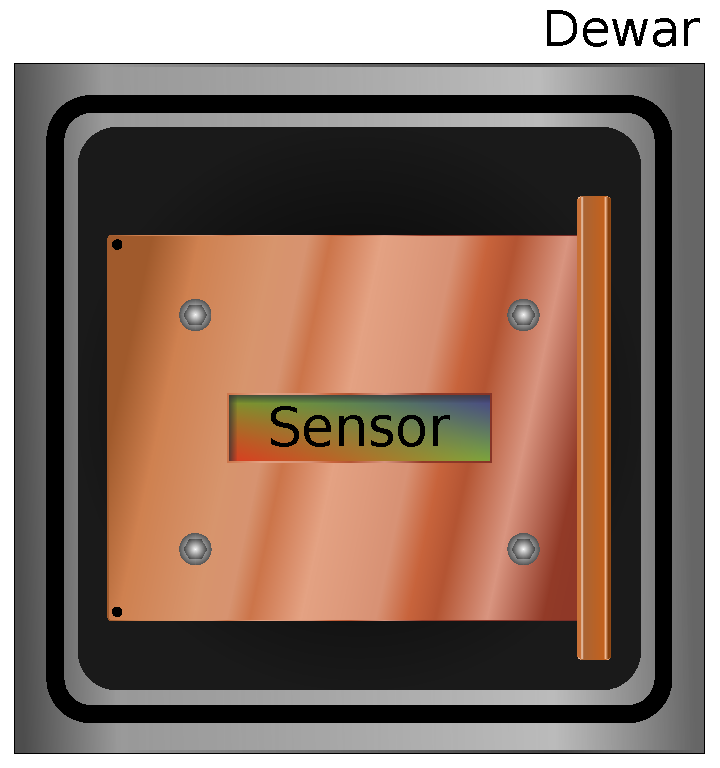
\includegraphics[scale=0.5]{Figs/Frontal_Dewar_Sensor.pdf}
    \caption{Esquema frontal del \textit{dewar} y el posicionamiento del sensor. El sensor se encuentra montado detrás de una placa de cobre frontal con un abertura rectangular por donde la radiación incidente alcanza al sensor. A su vez, se cubren las esquinas laterales del sensor con dos láminas de cobre para evitar la exposición de esas regiones del CCD, donde es desplazada la carga para posteriormente ser medida.}
    \label{fig:FrontalDewarYSensor}
\end{figure}
Para evitar la condensación de humedad sobre la superficie del detector debido a las bajas temperaturas, se hizo vacío en el \textit{dewar} mediante la utilización de una bomba turbo-molecular capaz de alcanzar una presión del orden de los $10^{-5}\,\si{mbar}$.

También fue necesaria la utilización de un calentador eléctrico para controlar la temperatura del sensor por dos razones principales: evitar que la temperatura de operación del sensor sea menor a $110\,\si{K}$, debido a que la eficiencia de la transferencia de carga entre píxeles del sensor se ve disminuida para temperaturas menores a esta; y para regular la velocidad de enfriamiento del sensor, dado que podría comprometerse su integridad estructural si esta superaba $1\,\si{K/s}$.

%%%%%%%%%%%%%%%%%%%%%%%%%%%%%%%%%%%%%%%%%%%%%%%%%%%%%%%%%%%%%%%%%%
%%%%%%%%%%%%%%%%%%%%%%%%%%%%%%%%%%%%%%%%%%%%%%%%%%%%%%%%%%%%%%%%%%
\subsection{Fuente de \texorpdfstring{$\Am{241}$}{Am241}}
\noindent En las mediciones estudiadas en este trabajo, se utilizó una fuente radioactiva de $\Am{241}$ electrodepositada, que emitía partículas $\alpha$ con energía de $\sim 5.6\,\si{MeV}$, una actividad de $1\,\si{\mu C}$ y un diámetro de $5\,\si{mm}$. 
Para obtener los rayos $X$ de fluorescencia del flúor y del aluminio, se colocaron dentro de la caja de cobre, frente al sensor, una cinta de Teflón (material que contiene flúor), y una placa de aluminio. La fuente radioactiva se encontraba debajo de esta caja de cobre, a la cual se le hizo un orificio por donde ingresaban las partículas $\alpha$ que impactaban los materiales mencionados, como muestra el esquema de la Figura \ref{fig:FrontalAlYF}. Esto producía excitaciones en sus nubes electrónicas que luego, al desexcitarse, emitían los fotones de fluorescencia que alcanzaban al sensor.
\begin{figure}[h]
    \centering
    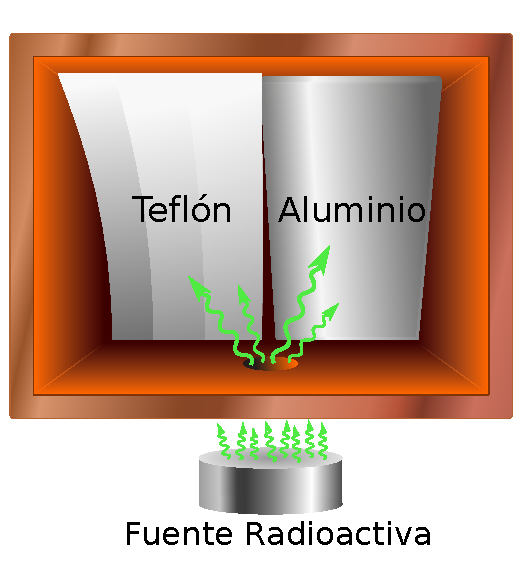
\includegraphics[scale=0.7]{Figs/CajaSensor.pdf}
    \caption{Esquema frontal de la caja de cobre donde se posicionaron la cinta de teflón y la placa de aluminio. Se esquematiza el orificio por donde ingresan las partículas alfa. El sensor se encuentra montado frente de esta, detrás de la placa de cobre del esquema de la Figura \ref{fig:FrontalDewarYSensor}, de forma que los rayos de fluorescencia producidos por el aluminio y el teflón impacten sobre él.}
    \label{fig:FrontalAlYF}
\end{figure}

En el esquema de la Figura \ref{fig:LateralDewar} puede verse un corte lateral de la cámara. Del lado derecho se encuentra la caja de cobre que contiene el material que se utiliza para producir los rayos $X$ (flúor o aluminio) y la fuente radioactiva emisora de partículas $\alpha$. 
Del lado izquierdo puede verse la estructura que sostiene el detector y la pieza de cobre destinada a regular la temperatura del mismo.

\begin{figure}%[h]
    \centering
    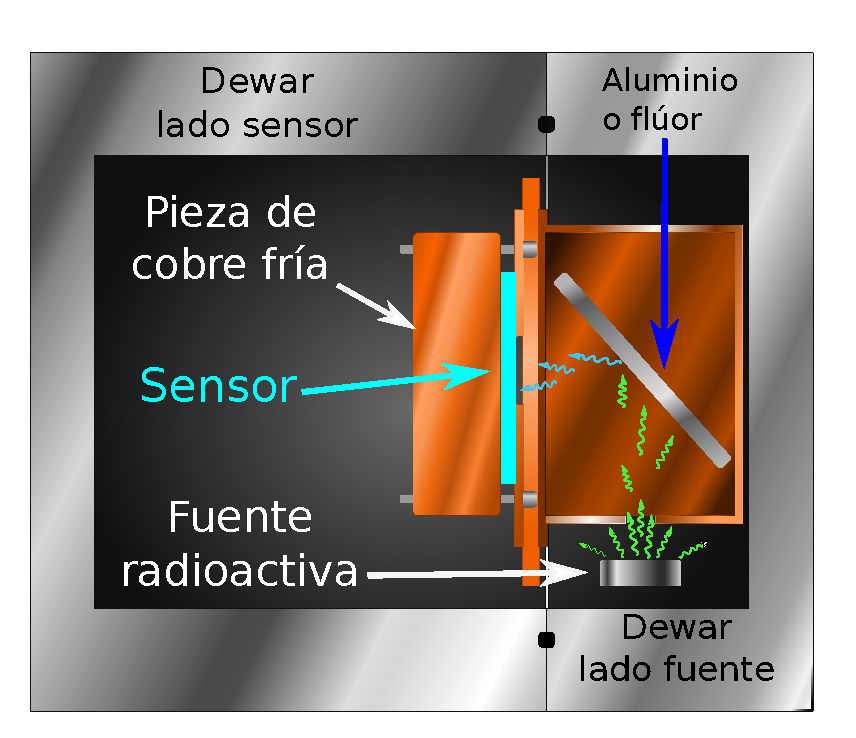
\includegraphics[scale=0.7]{Figs/LateralDewar.pdf}
    \caption{Esquema lateral del \textit{dewar}. Del lado izquierda se encuentra la placa de cobre con la abertura para el sensor (vista lateral del esquema \ref{fig:FrontalDewarYSensor}) el cual está en contacto con una pieza de cobre fría para mantenerlo a $123\,\si{K}$. Del lado derecho se encuentra la caja de cobre con la pieza de aluminio o de flúor, posicionada en ángulo y por encima del orificio por donde pasan las partículas alfa de la fuente radioactiva (vista lateral del esquema \ref{fig:FrontalAlYF}).}
    \label{fig:LateralDewar}
\end{figure}
Por otro lado, como los fotones de la fuente radioactiva eran capaces de impactar en cualquier parte de la superficie de la caja de cobre, este podría producir también fotones de fluorescencia. Para evitar esto se recubrió el interior de la caja de cobre con cinta \textit{Kapton}, la cual está compuesta por moléculas de bajo número atómico $Z$, que en caso de emitir fotones de fluorescencia, lo harían a energías menores a las de interés en este trabajo.
%\textcolor{red}{me quedé con la sensación de que era mejor contar todo esto al revés, primero el sensor, después la fuente radiactiva y por ultimo decir porque se pone la cámara}
%\textcolor{blue}{mover la fuente es más dificil porque hay que reformular y no me parece que amerite}

%%%%%%%%%%%%%%%%%%%%%%%%%%%%%%%%%%%%%%%%%%%%%%%%%%%%%%%%%%%%%%%%%%
%%%%%%%%%%%%%%%%%%%%%%%%%%%%%%%%%%%%%%%%%%%%%%%%%%%%%%%%%%%%%%%%%%

\section{Mediciones \label{sec:Mediciones}}

%\textcolor{red}{hay mucho para mejorar en esta sección que empieza. Varias cosas no son del todo correctas y la explicación no fluye.}\textcolor{blue}{Oka, para mi lo único flojardo es el párrafo que dice "de las $500$ columnas que tiene el sensor, se utilizaron... bla bla" porque eso es lo que no me quedó claro. Pero no veo qué le puede faltar a nivel explicación, yo siento que tiene lo que tiene que tener}

\noindent Las mediciones se realizaron exponiendo la mitad central del sensor a la radiación incidente y dejando las mitades laterales donde se encuentran los amplificadores cubiertos por láminas de cobre, como se ve en el esquema de la Figura \ref{fig:FrontalDewarYSensor}, de forma de evitar su exposición. Los cuatro cuadrantes del sensor son expuestos por un breve período de tiempo a la radiación (decenas de milisegundos), para rápidamente desplazar la carga colectada a la zona del sensor cubierta por las láminas de cobre y evitar que siga recibiendo interacciones durante el proceso de lectura. %, el cual tomaba aproximadamente $11$ minutos.
Este procedimiento es importante porque si no se mueve la carga rápidamente a la región cubierta, la actividad de la fuente saturaría de eventos el detector haciendo imposible la diferenciación de eventos en las imágenes.

%Es importante notar que el tiempo que se demora en desplazar la carga de la región expuesta a la región cubierta depende de la cantidad de columnas del sensor que se quieren medir. Si por ejemplo, quieren medirse $50$ columnas, la columna número $50$ abandonará la región expuesta en un tiempo $t$. Pero si lo que se quiere medir son $100$ columnas, entonces en este caso la columna número $100$ abandonará la región expuesta en un tiempo $\sim 2t$. Esto implica que la cantidad de eventos medidos es proporcional a la cantidad de columnas que se quieran medir además de que las últimas columnas tendrán cada vez más eventos.

%\noindent Debido a que la tasa de eventos de fluorescencia de aluminio y flúor producidos fue relativamente baja, las colección de eventos se realizó exponiendo el detector durante $20$ minutos antes de realizar la medición de la carga en los píxeles. 
Luego, para las mediciones de la carga se utilizaron $300$ muestreos por píxel, que corresponde a un tiempo de lectura de aproximadamente $11$ minutos por imagen. En cada una de ellas fueron utilizadas $50$ filas del sensor, donde para cada una se midieron $500$ píxeles, de los cuales $7$ fueron de \textit{pre-scan}, $50$ de \textit{over-scan} y $443$ de región activa. El \textit{pre-scan} son píxeles adicionales del registro horizontal, cuyo fin es el de proveer un retardo para que la señal de video se estabilice y así poder realizar adecuadamente las mediciones subsiguientes. El \textit{over-scan}, por su parte, también corresponde a píxeles adicionales del registro horizontal: si el registro horizontal cuenta con $443$ píxeles, cuando el primer píxel con carga es desplazado hacia nodo de sensado, quedarán $442$ píxeles con carga por leer y un píxel vacío al final. Este es el primer píxel del \textit{over-scan}. Cuando el segundo píxel con carga es desplazado hacia el nodo de sensado, quedarán $441$ píxeles por leer y 2 píxeles vacíos al final, con lo cual ahora hay 2 píxeles de \textit{over-scan}. De esta forma, a medida que se van leyendo los píxeles de la fila, se van vaciando píxeles al final, que a su vez son desplazados junto con los píxeles con carga hacia el nodo de sensado. Esto hace que el tiempo de exposición a las interacciones de estos píxeles sea mucho más menor y, por ende, la probabilidad de capturar carga de estos es muy baja.

%pero cuando se realiza la medición de los píxeles y las cargas son desplazadas secuencialmente, estos se ven obligados a atravesar la región del sensor que está expuesta a la radiación y en consecuencia tienen una probabilidad no nula, aunque muy baja, de colectar algún evento al moverse hacia el nodo de sensado. 

Luego de la lectura, las $300$ mediciones tomadas para cada píxel fueron promediadas y los píxeles del \textit{over-scan}, debido a su baja probabilidad de colectar carga durante el proceso de lectura, fueron usados para calcular y extraer la linea de base de cada fila. Este proceso es necesario en la calibració para poder establecer el valor en ADU's correspondiente al $0$ de carga para cada una de las filas del sensor. 

%Luego de la lectura, las $300$ mediciones tomadas para cada píxel fueron promediadas y los píxeles vacíos del \textit{over-scan} fueron usados para calcular y extraer la linea de base de cada fila. Este proceso es necesario para la calibración, para poder establecer el valor en ADU's correspondiente al $0$ de carga para cada una de las filas del sensor. 

%Las regiones de \textit{pre-scan} y \textit{over-scan} son regiones del sensor que no están colectando carga junto con la región activa, pero cuando se realiza la medición de los píxeles y las cargas son desplazadas secuencialmente, estos píxeles atraviesan la región del sensor expuesta y en consecuencia tienen una probabilidad no nula, aunque muy baja, de colectar algún evento al desplazarse hacia el nodo de sensado. 

%Esa baja probabilidad de colectar carga durante el proceso de lectura es la razón por la cual esos píxeles son utilizadas para definir la linea de base de cada fila. Al final de cada ciclo de exposición/lectura, toda la carga colectada por el CCD era removida en un rápido proceso que toma aproximadamente un segundo.

Las imágenes resultantes luego de la medición y el promediado contienen $50 \times 500$ píxeles por cada cuadrante y la carga es medida en unidades electrónico digitales (ADU's), que posteriormente son convertidas en electrones usando la calibración absoluta del sensor.